\documentclass[a4paper,11pt]{article}

% ─── Packages ────────────────────────────────────────────────────
\usepackage[utf8]{inputenc}
\usepackage[T1]{fontenc}
\usepackage[margin=2.5cm]{geometry}
\usepackage{xcolor}
\usepackage{listings}
\usepackage{tcolorbox}
\usepackage{graphicx}
\usepackage{titlesec}
\usepackage{hyperref}
\usepackage{fancyhdr}
\usepackage{multicol}

% ─── Style Definitions ───────────────────────────────────────────
\definecolor{lightgray}{rgb}{.9,.9,.9}
\definecolor{darkgray}{rgb}{.4,.4,.4}
\definecolor{purple}{rgb}{0.65, 0.12, 0.82}
\definecolor{codegreen}{rgb}{0,0.6,0}
\definecolor{codegray}{rgb}{0.5,0.5,0.5}
\definecolor{codepurple}{rgb}{0.58,0,0.82}
\definecolor{backcolour}{rgb}{0.95,0.95,0.92}
\definecolor{pastelblue}{HTML}{E3F2FD}
\definecolor{pastelpink}{HTML}{FCE4EC}
\definecolor{pastelgreen}{HTML}{E8F5E9}

\tcbuselibrary{skins,breakable}

\lstdefinelanguage{JavaScript}{
  keywords={break, case, catch, continue, debugger, default, delete, do, else, false, finally, for, function, if, in, instanceof, new, null, return, switch, this, throw, true, try, typeof, var, void, while, with},
  morecomment=[l]{//},
  morecomment=[s]{/*}{*/},
  morestring=[b]',
  morestring=[b]",
  ndkeywords={class, export, boolean, throw, implements, import, this},
  keywordstyle=\color{blue}\bfseries,
  ndkeywordstyle=\color{darkgray}\bfseries,
  identifierstyle=\color{black},
  commentstyle=\color{codegreen}\ttfamily,
  stringstyle=\color{codepurple}\ttfamily,
  sensitive=true
}

\lstdefinelanguage{CSS}{
  keywords={color,background,margin,padding,font,weight,display,position,top,left,right,bottom,list,style,border,size,white,space,min,width,transition, transform, transition-property, transition-duration, transition-timing-function, border-radius, box-shadow},
  sensitive=true,
  morecomment=[l]{//},
  morecomment=[s]{/*}{*/},
  morestring=[b]',
  morestring=[b]",
  keywordstyle=\color{blue}\bfseries,
  commentstyle=\color{codegreen}\ttfamily,
  stringstyle=\color{codepurple}\ttfamily
}

\newtcolorbox{explanationbox}[1]{
  colback=pastelblue,
  colframe=blue!50!black,
  fonttitle=\bfseries,
  title=#1,
  arc=5mm,
  breakable,
  enhanced,
  drop shadow
}

\lstdefinestyle{mystyle}{
    backgroundcolor=\color{backcolour},   
    commentstyle=\color{codegreen},
    keywordstyle=\color{magenta},
    numberstyle=\tiny\color{codegray},
    stringstyle=\color{codepurple},
    basicstyle=\ttfamily\footnotesize,
    breakatwhitespace=false,         
    breaklines=true,                 
    captionpos=b,                    
    keepspaces=true,                 
    numbers=left,                    
    numbersep=5pt,                  
    showspaces=false,                
    showstringspaces=false,
    showtabs=false,                  
    tabsize=2
}

\lstset{style=mystyle}

% ─── Metadata ────────────────────────────────────────────────────
\title{SignBridge: The Ultimate Codebase Deep Dive}
\author{Documentation Agent \& Cute Robots}
\date{\today}

\begin{document}

\maketitle
\begin{center}
    
\includegraphics[width=0.4\textwidth]{doodles/fun-emoji_1.pdf}
\end{center}
\newpage
\tableofcontents
\newpage

\section{Chapter 1: Project Architecture \& Environment}
Welcome to the inner workings of SignBridge! This chapter sets the stage by explaining the "big picture" of how various technologies come together to turn hand gestures into words.

\begin{explanationbox}{The Tech Stack Philosophy}
SignBridge is built on a foundation of "Perception-First" engineering. We prioritize low-latency hand tracking above all else.
\begin{itemize}
    \item \textbf{MediaPipe}: Our eyes. It provides 21 high-fidelity 3D hand landmarks at 30+ FPS.
    \item \textbf{Scikit-learn}: Our brain. A Random Forest Classifier interprets these landmarks.
    \item \textbf{Flask-SocketIO}: Our central nervous system. It bridges the gap between Python's processing power and the web browser's reactivity.
\end{itemize}
\end{explanationbox}

\begin{center}
    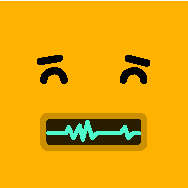
\includegraphics[width=0.2\textwidth]{doodles/bottts-neutral_1.pdf}
\end{center}

\subsection{Hardware-Software Interface}
One of the most unique features of SignBridge is its integration with physical hardware. We use a Raspberry Pi Pico (connected via USB Serial) to display the translated text on an OLED screen. This allows the system to be used even without looking at a monitor!

\begin{explanationbox}{Serial Communication}
We use the \texttt{pyserial} library to talk to the Pico. The protocol is simple but effective: we send strings formatted as \texttt{CMD:VALUE}. For example, \texttt{LETTER:A} tells the Pico to show a large 'A' on its display.
\end{explanationbox}

% --- collectdata.py ---
\section{Chapter 2: The Data Acquisition Pipeline}
Before we can translate, we must learn. This chapter explains \texttt{collectdata.py}, the tool used to build our custom sign language dataset.

\subsection{Initialization and Setup}
\begin{explanationbox}{The Import Block}
Every Python script starts here. We import \texttt{cv2} for camera access and \texttt{mediapipe} for the heavy lifting of hand detection.
\end{explanationbox}
\begin{lstlisting}[language=Python]
import os
import cv2
import mediapipe as mp
import csv
import numpy as np
\end{lstlisting}

\begin{explanationbox}{Sign List and Sample Size}
We define which signs we want to record. By default, it's A-Z plus some special words like "HELP" and "THANKS". We record 100 samples per sign to ensure the model sees enough variations in hand positioning.
\end{explanationbox}
\begin{lstlisting}[language=Python]
SIGNS = list("ABCDEFGHIJKLMNOPQRSTUVWXYZ") + ["NAMASTE", "YES", "NO", "HELP", "THANKS"]
SAMPLES_PER_SIGN = 100
\end{lstlisting}

\begin{center}
    
\includegraphics[width=0.2\textwidth]{doodles/thumbs_1.pdf}
\end{center}

\subsection{Configuring MediaPipe Hands}
\begin{explanationbox}{Static Image Mode}
In \texttt{collectdata.py}, we set \texttt{static\_image\_mode=True}. This is a "pro tip": when recording individual samples, this mode tells MediaPipe to treat every frame as a fresh start, resulting in higher detection accuracy at the cost of some processing speed.
\end{explanationbox}
\begin{lstlisting}[language=Python]
mp_hands = mp.solutions.hands
hands = mp_hands.Hands(
    static_image_mode=True,
    max_num_hands=1,
    min_detection_confidence=0.5,
)
\end{lstlisting}

\subsection{Webcam Management}
\begin{explanationbox}{The open\_camera Function}
Webcams can be tricky. This function iterates through indices [1, 0] to find an active camera. It also performs a "smoke test" by reading a single frame before returning the capture object.
\end{explanationbox}
\begin{lstlisting}[language=Python]
def open_camera():
    for idx in [1, 0]:
        cap = cv2.VideoCapture(idx)
        if cap.isOpened():
            ret, test = cap.read()
            if ret and test is not None:
                print(f"Camera opened on index {idx}")
                return cap
            cap.release()
    raise RuntimeError("No camera found!")
\end{lstlisting}

\subsection{The Interactive Capture Loop}
\begin{explanationbox}{{Ready, Set, Record!}}
The script guides the user through each sign. It waits for the user to press SPACE before starting the high-speed recording of 100 landmark sets.
\end{explanationbox}
\begin{lstlisting}[language=Python]
for sign in SIGNS:
    # ... Wait for SPACE key ...
    while count < SAMPLES_PER_SIGN:
        # ... Capture Frame ...
        rgb = cv2.cvtColor(frame, cv2.COLOR_BGR2RGB)
        result = hands.process(rgb)
\end{lstlisting}

\begin{center}
    
\includegraphics[width=0.25\textwidth]{doodles/fun-emoji_2.pdf}
\end{center}

\begin{explanationbox}{Saving Landmarks to CSV}
When a hand is detected, we extract the $(x, y, z)$ coordinates for all 21 landmarks. This gives us 63 numerical features per frame. We save these, along with the sign label, into \texttt{data/landmarks.csv}.
\end{explanationbox}
\begin{lstlisting}[language=Python]
        if result.multi_hand_landmarks:
            lm = result.multi_hand_landmarks[0].landmark
            row = [sign] + [v for p in lm for v in (p.x, p.y, p.z)]
            samples.append(row)
            count += 1
\end{lstlisting}

\newpage
% --- trainmodel.py ---
\section{Chapter 3: The Machine Learning Engine}
Now that we have our data, we need to train a model that can generalize to new, unseen hand positions. This chapter covers \texttt{trainmodel.py}.

\subsection{Theoretical Basis: Landmark Normalization}
\begin{explanationbox}{Why Normalize?}
Raw MediaPipe landmarks are absolute pixel coordinates (or relative to frame size). If you move your hand to the corner of the screen, the numbers change completely, even if you're making the same sign. Normalization fixes this.
\end{explanationbox}

\begin{lstlisting}[language=Python]
def normalize_landmarks(raw):
    """Normalize relative to wrist (landmark 0), scale to unit range."""
    bx, by, bz = raw[0], raw[1], raw[2]
    norm = []
    for i in range(0, len(raw), 3):
        norm.extend([raw[i] - bx, raw[i + 1] - by, raw[i + 2] - bz])
    m = max(abs(v) for v in norm)
    if m > 0:
        norm = [v / m for v in norm]
    return norm
\end{lstlisting}

\begin{explanationbox}{The Logic in Depth}
1. \textbf{Translation}: We treat the wrist (landmark 0) as the origin $(0,0,0)$. By subtracting the wrist's coordinates from every other landmark, we make the model \textbf{position-invariant}.
2. \textbf{Scaling}: We find the maximum absolute value among all relative coordinates and divide everything by it. This scales the hand to fit inside a $[-1, 1]$ cube, making the model \textbf{scale-invariant} (robust to hand distance).
\end{explanationbox}

\begin{center}
    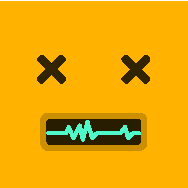
\includegraphics[width=0.25\textwidth]{doodles/bottts-neutral_2.pdf}
\end{center}

\subsection{Data Augmentation for Robustness}
\begin{explanationbox}{Simulating Real-World Noise}
Real hand tracking is never perfect. To prevent the model from overfitting to "perfect" landmarks, we inject small amounts of Gaussian noise into our training data.
\end{explanationbox}
\begin{lstlisting}[language=Python]
for i in range(len(norm_data)):
    for _ in range(3):  # 3 augmented copies per sample
        noisy = np.array(norm_data[i]) + np.random.normal(0, 0.02, len(norm_data[i]))
        aug_norm_data.append(noisy.tolist())
        aug_labels.append(labels[i])
\end{lstlisting}

\subsection{The Random Forest Classifier}
\begin{explanationbox}{Why Random Forest?}
Random Forests are excellent for this task because they handle non-linear relationships well and are resistant to noise. With 300 decision trees, our model becomes highly reliable.
\end{explanationbox}
\begin{lstlisting}[language=Python]
model = RandomForestClassifier(
    n_estimators=300,       # more trees = more stability
    max_depth=None,         # grow fully for max detail
    min_samples_leaf=1,     
    max_features='sqrt',    # helps decorrelate the trees
    random_state=42,
    n_jobs=-1,              # parallel processing
)
model.fit(X_train, y_train)
\end{lstlisting}

\begin{center}
    
\includegraphics[width=0.3\textwidth]{doodles/thumbs_2.pdf}
\end{center}

\subsection{Model Evaluation and Persistence}
After training, we evaluate the model using accuracy scores and cross-validation. Finally, we save the trained object using \texttt{pickle}.
\begin{lstlisting}[language=Python]
with open("model.pkl", "wb") as f:
    pickle.dump(model, f)
\end{lstlisting}

\newpage
% --- app.py Part 1 ---
\section{Chapter 4: The Real-Time Translation Core (Part 1)}
\texttt{app.py} is a masterclass in combining high-performance vision with thread-safe web serving. This chapter explores how we manage state and the Finite State Machine (FSM).

\subsection{Architectural Design: The AppState Class}
\begin{explanationbox}{Why a Shared State?}
In a real-time translator, one thread is constantly capturing frames from the camera, while another thread (the Flask server) is answering requests from the user's browser. If both threads try to update the same variable at the same time, the app will crash. \texttt{AppState} solves this with a \textbf{Thread Lock}.
\end{explanationbox}

\begin{lstlisting}[language=Python]
class AppState:
    def __init__(self):
        self._lock = threading.Lock()
        self.hand_detected = False
        self.raw_prediction = ""
        # ... other variables ...
\end{lstlisting}

\begin{explanationbox}{Thread Safety in Action}
Every time the camera thread wants to update the prediction, it must first "acquire" the lock. This ensures that the Flask server won't read a half-written variable.
\end{explanationbox}
\begin{lstlisting}[language=Python]
    def update_detection(self, hand_detected, raw_pred, raw_conf, fsm_state, cooldown, proposal=""):
        with self._lock: # The magic happens here!
            self.hand_detected = hand_detected
            self.raw_prediction = raw_pred
            self.raw_confidence = raw_conf
            self.fsm_state = fsm_state
            self.cooldown_remaining = cooldown
            self.proposal = proposal
\end{lstlisting}

\begin{center}
    
\includegraphics[width=0.25\textwidth]{doodles/fun-emoji_3.pdf}
\end{center}

\subsection{The Finite State Machine (FSM)}
\begin{explanationbox}{Defining the User Experience}
To make the translator feel "intelligent," we use an FSM. This determines what the UI shows based on confidence and timing.
\end{explanationbox}

\begin{explanationbox}{FSM States}
\begin{itemize}
    \item \textbf{Idle}: No hand is visible. The system is resting.
    \item \textbf{Detecting}: A hand is seen, and we are actively voting on the sign.
    \item \textbf{Locked}: A letter was just confirmed. We pause for 1.2 seconds so the user can transition to the next sign without accidentally confirming the same letter twice.
    \item \textbf{Waiting}: The hand is seen, but confidence is low. We show a "WAIT" message to the user.
\end{itemize}
\end{explanationbox}

\begin{lstlisting}[language=Python]
        # Determine FSM state in the main loop
        if not hand_detected:
            fsm = "idle"
        elif in_cooldown:
            fsm = "locked"
        elif raw_conf < CONF_FLOOR:
            fsm = "waiting"
        else:
            fsm = "detecting"
\end{lstlisting}

\begin{center}
    
\includegraphics[width=0.3\textwidth]{doodles/bottts-neutral_3.pdf}
\end{center}

\newpage
% --- app.py Part 2 ---
\section{Chapter 4: The Real-Time Translation Core (Part 2)}
In this section, we dive into how SignBridge makes final decisions and communicates them to the world.

\subsection{Temporal Stabilization: Majority Voting}
\begin{explanationbox}{Defeating the Jitter}
Single-frame predictions are often jumpy. If the model is 51\% sure it's an 'A' and 49\% sure it's an 'E', the UI would flicker between them. We solve this by looking at a \textbf{Sliding Window} of 8 frames.
\end{explanationbox}

\begin{lstlisting}[language=Python]
vote_buffer = deque(maxlen=VOTE_WINDOW) # VOTE_WINDOW = 8

# Check for letter confirmation
if hand_detected and not in_cooldown and len(vote_buffer) >= VOTE_THRESHOLD:
    valid_votes = [v for v in vote_buffer if v is not None]
    if len(valid_votes) >= VOTE_THRESHOLD:
        counter = Counter(valid_votes)
        top_sign, top_count = counter.most_common(1)[0]
        if top_count >= VOTE_THRESHOLD and top_sign != last_confirmed:
            # Letter is confirmed!
            state.confirm_letter(top_sign)
\end{lstlisting}

\begin{explanationbox}{The Consensus Rule}
A letter is only added to the word if \textbf{6 out of the last 8 frames} show the exact same sign. This "consensus" rule makes the translation feel solid and reliable.
\end{explanationbox}

\begin{center}
    
\includegraphics[width=0.25\textwidth]{doodles/thumbs_3.pdf}
\end{center}

\subsection{Intelligent Auto-completion with PrefixTrie}
\begin{explanationbox}{Why a Trie?}
Searching for words in a list of 75,000 items is slow. A \textbf{Trie} (prefix tree) allows us to find all words starting with "HE" in just a few microseconds.
\end{explanationbox}

\begin{lstlisting}[language=Python]
class TrieNode:
    def __init__(self):
        self.children = {}
        self.is_word = False

class PrefixTrie:
    def search_prefix(self, prefix, limit=3):
        prefix = prefix.upper()
        node = self.root
        for char in prefix:
            if char not in node.children:
                return [] # Prefix not found
        # ... DFS to find completions ...
\end{lstlisting}

\subsection{The Communication Layer: REST \& WebSockets}
\begin{explanationbox}{Hybrid Communication}
SignBridge uses two types of communication:
\begin{enumerate}
    \item \textbf{WebSockets (SocketIO)}: For high-speed data that updates every 100ms (like the hand confidence ring).
    \item \textbf{REST API (Flask)}: For discrete actions like pressing the "Clear" button or requesting a sentence completion.
\end{enumerate}
\end{explanationbox}

\begin{lstlisting}[language=Python]
@app.route("/action/clear", methods=["POST"])
def action_clear():
    state.clear_sentence()
    send_to_pico("CLEAR")
    socketio.emit("state_update", state.get_snapshot())
    return jsonify({"ok": True})
\end{lstlisting}

\newpage
% --- Frontend ---
\section{Chapter 5: Human-Interface \& Visualization}
The frontend is where the machine learning magic becomes a usable product. We've designed it to be both visually striking and highly functional.

\subsection{Neobrutalist Design Philosophy}
\begin{explanationbox}{Why Neobrutalism?}
Neobrutalism uses high contrast, bold black borders, and vibrant colors. This isn't just for looks—it makes the UI elements (like the letter tiles) extremely distinct and easy to read from a distance.
\end{explanationbox}

\begin{lstlisting}[language=CSS]
/* The signature Neobrutalist Shadow */
.card {
    background: var(--card-bg);
    border: var(--border); /* 0.5rem solid black */
    box-shadow: 1rem 1rem 0px #000000;
    transition: all 0.1s;
}

.card:hover {
    transform: translate(-4px, -4px);
    box-shadow: 1.25rem 1.25rem 0px #000;
}
\end{lstlisting}

\begin{center}
    
\includegraphics[width=0.25\textwidth]{doodles/fun-emoji_1.pdf}
\end{center}

\subsection{Reactive UI with SocketIO}
\begin{explanationbox}{Instant Feedback}
When the backend confirms a letter, the frontend needs to know immediately. We use \texttt{socket.on} to listen for events and update the DOM in real-time.
\end{explanationbox}

\begin{lstlisting}[language=JavaScript]
// Listening for state updates
socket.on("state_update", (data) => {
    updateUI(data); // Re-renders the hand indicator, ring, and tiles
});

// High-impact confirmation animation
socket.on("letter_confirmed", (data) => {
    // Cobalt Blue high-impact flash!
    document.body.style.backgroundColor = "var(--accent-blue)";
    setTimeout(() => {
        document.body.style.backgroundColor = "var(--bg)";
    }, 100);
});
\end{lstlisting}

\section{Chapter 6: Conclusion \& Future Work}
\begin{explanationbox}{Project Wrap-up}
SignBridge demonstrates how complex AI can be made accessible through thoughtful software engineering and creative design. By combining MediaPipe, Scikit-learn, and modern web tech, we've built a bridge between two worlds.
\end{explanationbox}

\begin{center}
    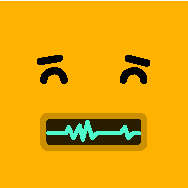
\includegraphics[width=0.4\textwidth]{doodles/bottts-neutral_1.pdf}
\end{center}

\subsection{What's Next?}
The current system is excellent for finger-spelling. Future versions will incorporate \textbf{Long Short-Term Memory (LSTM)} networks to recognize fluid, whole-word signs (like "Thank you" or "Goodbye") by analyzing sequences of frames over time.

\newpage
\end{document}




